\section{Research Methods}
\label{sec:research-methodology:review}

Research methods are ``a set of organising principles around which empirical data is collection and analysed'' \citep{Easterbrook:2007ws}. \citet{Creswell:2017vn} suggests that strong research design is reflected when the weaknesses of multiple methods complement each other. Using a mixed-methods approach is therefore commonplace in software engineering research, typically due to the human-oriented nature investigating how software engineers work both individually (where methods from psychology may be employed) and together (where methods from sociology may be employed).

Therefore, studies in software engineering are typically performed as field studies where researchers and developers (or the artefacts they produce) are analysed either directly or indirectly \citep{Singer:2007tu}. The mixed-methods approach combines five classes of field study methods (or empirical strategies/studies) most relevant in empirical software engineering research \citep{Easterbrook:2007ws, Wohlin:2012bu, Juristo:2013vj}: controlled experiments, case studies, survey research, ethnographies, and action research. We chiefly adopt a mixed-methods approach to our work using the \textit{concurrent triangulation} mixed-methods strategy \citep{Jick:1979el} as it best compensates for weaknesses that exist in all research methods, and employs the best strengths of others \citep{Creswell:2017vn}.

\subsection{Review of Relevant Research Methods}
\label{ssec:research-methodology:review:methods}

Below we review some of the research methods most relevant to our research questions as refined in \cref{sec:research-methodology:research-questions} as presented by \citet{Easterbrook:2007ws}.

\subsubsection{Controlled Experiments}
A controlled experiment is an investigation of a clear, testable hypothesis that guides the researcher to decide and precisely measure how at least one independent variable can be manipulated and effect at least one other dependent variable. They determine if the two variables are related and if a cause-effect relationship exists between them. The combination of independent variable values is a \textit{treatment}. It is common to recruit human subjects to perform a task and measure the effect of a randomly assigned treatment on the subjects, though it is not always possible to achieve full randomisation in real-life software engineering contexts, in which case a \textit{quasi-experiment} may be employed where subjects are not randomly assigned to treatments.

While we have well-defined RQs, refining them into precise, \textit{measurable} variables is challenging due to the qualitative nature they present. A well-defined population is also critical and must be easily accessible; the varied range of beginner to expert software engineers with varied understanding of artificial intelligence concepts is required to perform controlled experiments, and thus recruitment may prove challenging. Lastly, the controlled experiment is essentially reductionist by affecting a small amount of variables of interest and controlling all others. This approach is too clinical for the practical outcomes by which our research goals aim for, and is therefore closely tied to the positivist stance.

\subsubsection{Case Studies}
Case studies investigate phenomena in their real-life context and are well-suited when the boundary between context and phenomena is unknown \citep{Yin:2017tf}. They offer understanding of how and why certain phenomena occur, thereby investigating ways cause-effect relationships can occur. They can be used to test existing theories (\textit{confirmatory case studies}) by refuting theories in real-world contexts instead of under laboratory conditions or to generate new hypotheses and build theories during the initial investigation of some phenomena (\textit{exploratory case studies}).

Case studies are well-suited where the context of a situation plays a role in the phenomenon being studied. They also lend themselves to purposive sampling rather than random sampling, and thus it is possible to selectively choose cases that benefit our research goals and (using our critical theorist stance) select cases that will actively benefit our participant software engineering audience most to draw attention to situations regarded as problematic in \gls{cvs}.

\subsubsection{Survey Research}
Survey research identifies characteristics of a broad population of individuals through direct data collection techniques such as interviews and questionnaires or independent techniques such as data logging. Defining that well-defined population is critical, and selecting a representative sample from it to generalise the data gathered usually assists in answering base-rate questions.

By identifying representative sample of the population, from beginner to experienced developers with varying understanding of \gls{cvs} \glspl{api}, we can use survey research to assist in answering our exploratory and base-rate RQs (see \cref{ssec:research-methodology:research-questions:empirical}) in determining the qualitative aspects of how individual developers perceive and work with the existing \glspl{api}, either by directly asking them, or by mining third-party discussion websites such as \glsx{so}. Similarlly, we can use this strategy to assess the developer's understanding on what makes \gls{api} documentation sufficient by assessing whether specific factors suggested from literature are useful according to developers. However, with direct survey research techniques, low response rates may prove challenging, especially if no inducements can be offered for participation.

\subsubsection{Ethnographies}
Ethnographies investigates the understanding of social interaction within community through field observation \citep{Robinson:2007tp}. Resulting ethnographies help understand how software engineering technical communities build practices, communication strategies and perform technical work collaboratively.

Ethnographies require the researcher to be highly trained in observational and qualitative data analysis, especially if the form of ethnography is participant observation, whereby the researcher is embedded of the technical community for observation. This may require the longevity of the study to be far greater than a couple of weeks, and the researcher must remain part of the project for its duration to develop enough local theories about how the community functions. While it assists in revealing subtle but important aspects of work practices within software teams, this study does not focus on the study of teams, and is therefore not a research method relevant to this project.


\subsubsection{Action Research}
Action researchers simultaneously solve real-world problems while studying the experience of solving the problem \citep{Davison:2004wo} by actively seeking to intervene in the situation for the purpose of improving it. A precondition is to engage with a \textit{problem owner} who is willing to collaborate in identifying and solving the problem faced. The problem must be authentic (a problem worth solving) and must have new knowledge outcomes for those involved. It is also characterised as an iterative approach to problem solving, where the knowledge gained from solving the problem has a desirable solution that empowers the problem owner and researcher.

This research is most associated to our adopted philosophical stance of critical theory. As this project is being conducted under the \gls{a2i2} collaboratively with engaged industry clients, we have identified a need for solving an authentic problem that industry faces. The desired outcome of this project is to facilitate wider change in the usage and development of \glspl{cvs}; thus, engaging action research as a potential method throughout the mixed-methods approach is used in this research.

\subsection{Review of Data Collection Techniques for Field Studies}
\label{ssec:research-methodology:review:techniques}

\citeauthor{Singer:2007tu} developed a taxonomy \citep{Singer:2007tu,Lethbridge:2005jv} showcasing data collection techniques in field studies that are used in conjunction with a variety of methods based on the level of interaction between researcher and software engineer, if any. This taxonomy is reproduced in \cref{fig:research-methodology:review:field-techniques}.

\begin{table}[p]
\centering
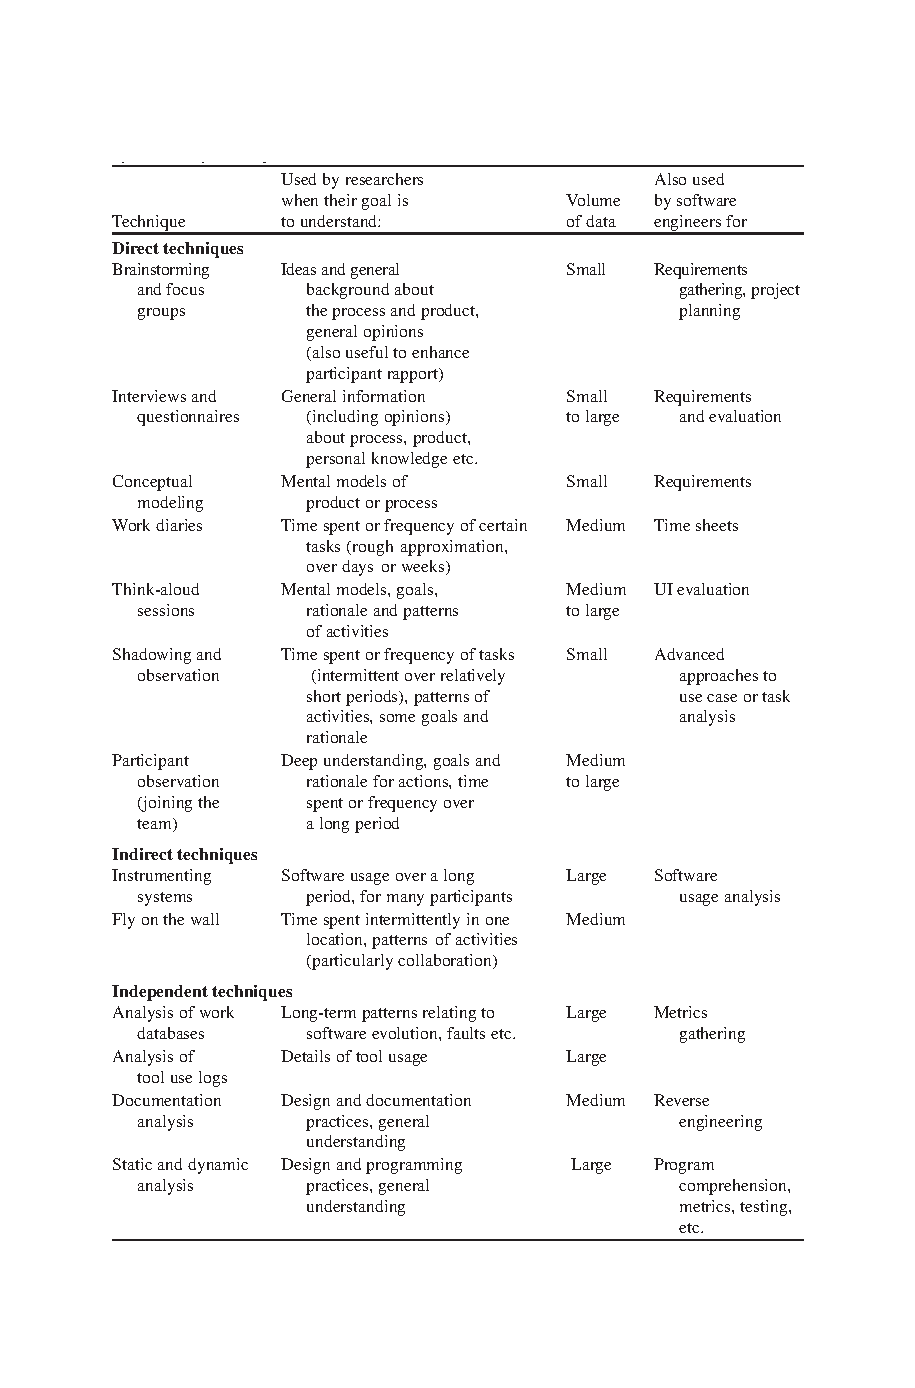
\includegraphics[width=0.95\linewidth]{mainmatter/research-methodology/figures/field-techniques}
\caption[Review of field study techniques]{Questions asked by software engineering researchers (column 2) that can be answered by field study techniques. (From \citep{Singer:2007tu}.)}
\label{fig:research-methodology:review:field-techniques}
\end{table}
